\section{Methodology}

Using FlexHeap, we perform a series of experiments to evaluate: 
(1) how FlexHeap compares to the baseline TeraHeap system without dynamic heap resizing,
(2) the impact of dynamic resizing on garbage collection overhead and
(3) the reduction in I/O traffic to the secondary heap device (H2).
These metrics allow us to assess both runtime performance and DRAM utilization efficiency.

Our experiments run on a high-performance dual-socket Intel server.
The system is equipped with two Intel Xeon Gold 5318Y CPUs, each with 24 physical cores 
and 2 hardware threads per core, for a total of 96 logical CPUs. It includes 256\,G of DRAM 
distributed across four NUMA nodes, with swap disabled. We co-locate all threads on a single
NUMA node to eliminate NUMA interference and use Linux cgroups to restrict the available DRAM,
enabling controlled and memory-constrained experiments.

For storage, we used two high-speed NVMe SSDs and one large-capacity SATA disk:
\begin{itemize}
  \item \texttt{/dev/nvme1n1}: a 1.8\,TB device formatted with \texttt{XFS}, used as the location of 
                               the H2 heap file for both Lucene and Spark workloads.
  \item \texttt{/dev/nvme2n1}: a 1.9\,TB device (\texttt{XFS}), used as the dataset disk for Lucene 
                               and the shuffle directory for Spark.
  \item \texttt{/dev/sda1}: a 3.6\,TB \texttt{EXT4} disk, used to store the Spark dataset.
\end{itemize}

All storage devices are directly attached with no RAID configuration. The operating system is Ubuntu 
24.04.1\,LTS with a Linux kernel version\,6.8.0-1020-nvidia.
\subsection{Lucene Methodology}

We evaluate our system using a real-world 200\,G Lucene index containing 52.6 billion words. 
To support the second-tier heap (H2), we preallocate a 300\,G file on NVMe storage, which serves as space 
for the query-cache to reside.
The dataset is preprocessed by removing stop words, single-character tokens, and non-English words. 
Terms are then grouped by frequency into two categories: high-frequency (top 1\%) and medium-frequency. 
High-frequency terms dominate document access patterns and generate significantly more I/O pressure.


We define two workloads:
\begin{itemize}[leftmargin=1.5em]
  \item \textbf{M1}: high-frequency small queries retrieving the top 50 results.
  \item \textbf{M2}: high-frequency large queries retrieving up to 500{,}000 results.
\end{itemize}

We run both M1 and M2 workloads under four DRAM budgets: 40\,G, 20\,G, 10\,G, and 8\,G,
enforced using Linux cgroups to control memory. 
For each DRAM setting, we evaluate both the static and a dynamic heap configuration. 
The static configuration, \textbf{TeraHeap}, evenly partitions the available DRAM between the 
managed heap (H1) and the page cache (H2), allocating 50\% of memory to each. In contrast, 
the dynamic configuration uses the \textbf{FlexHeap} policy, which adjusts the size of H1 
at runtime based on application behavior, while reserving a fixed 2\,G of DRAM for the page cache across all runs.

This setup allows us to evaluate the benefits of dynamic heap resizing under different memory constraints and workload pressures. 
The main heap (H1) sizes for different DRAM configurations are presented in Table~\ref{tab:lucene-configs}.

% \begin{table}[H]
% \centering
% \renewcommand{\arraystretch}{1.3}
% \caption{Lucene configurations for workloads M1 and M2 under.}
% \label{tab:lucene-configs}
% \begin{tabular}{|l|c|c|}
% \hline
% \textbf{Configuration} & \textbf{DRAM Budget} & \textbf{H1 / H2 Allocation (GiB)} \\
% \hline
% \multirow{4}{*}{TeraHeap (static)} 
%                        & 40\,G             & 20\,G / 20\,G \\
%                        & 20\,G             & 10\,G / 10\,G \\
%                        & 10\,G             & 5\,G / 5\,G   \\
%                        & 8\,G              & 4\,G / 4\,G   \\
% \hline
% \multirow{4}{*}{FlexHeap (dynamic)} 
%                        & 40\,G             & 38\,G / 2\,G  \\
%                        & 20\,G             & 18\,G / 2\,G  \\
%                        & 10\,G             & 8\,G / 2\,G   \\
%                        & 8\,G              & 6\,G / 2\,G   \\
% \hline
% \end{tabular}
% \end{table}

\begin{table}[H]
\centering
\renewcommand{\arraystretch}{1.1}
\caption{Lucene H1 size configurations for workloads M1 and M2.}
\label{tab:lucene-configs}
\begin{tabular}{|l|c|c|c|c|}

\hline
  \textbf{DRAM Budget} & 40\,G & 20\,G & 10\,G & 8\,G \\
\hline
  TeraHeap (static)& 20\,G & 10\,G & 5\,G & 4\,G \\
\hline
  FlexHeap (dynamic)& 38\,G & 18\,G  & 8\,G & 6\,G \\
\hline
 
\end{tabular}
\end{table}

\subsection{Spark Methodology}
\label{sec:spark-methodology}

We evaluate our dynamic heap resizing mechanism using a set of Spark workloads 
from the \texttt{spark-bench} suite. The selected benchmarks consist of:
(\texttt{PageRank}, \texttt{ConnectedComponent}, \texttt{ShortestPaths}, \texttt{TriangleCount}) 
and machine learning tasks (\texttt{SVDPlusPlus}, \texttt{LinearRegression}, \texttt{LogisticRegression}).

Similarly to Lucene, in the \textbf{TeraHeap} setup, the DRAM is partitioned statically between the managed heap (H1) and the second-tier 
storage-backed heap (H2), with allocation ratios manually chosen for each individual workload. In contrast, \textbf{FlexHeap} 
dynamically adjusts the size of H1 during execution, reserving part of the available DRAM for the page cache depending on
the runtime requirements of each benchmark. 

The total DRAM budget is workload-specific and chosen for each benchmark.
The heap allocations for both TeraHeap and FlexHeap configurations are summarized in Table~\ref{tab:spark-benchmark-configs}.
This setup enables us to evaluate how static versus dynamic DRAM partitioning impacts performance across different Spark tasks.

\begin{table}[htbp]
\centering
\small
\renewcommand{\arraystretch}{0.8}
\caption{Spark benchmark configurations under TeraHeap (static) and FlexHeap (dynamic).}
\label{tab:spark-benchmark-configs}
\begin{tabular}{|l|l|c|}
\hline
\textbf{Configuration} & \textbf{Benchmark} & \textbf{H1/page-cache (G)} \\
\hline
\multirow{7}{*}{TeraHeap (static)} 
& PageRank             & 64\,G / 16\,G \\
& ConnectedComponent   & 68\,G / 16\,G \\
& ShortestPaths        & 42\,G / 16\,G \\
& TriangleCount        & 64\,G / 16\,G \\
& SVDPlusPlus          & 24\,G / 16\,G \\
& LinearRegression     & 54\,G / 16\,G \\
& LogisticRegression   & 54\,G / 16\,G \\
\hline
\multirow{7}{*}{FlexHeap (dynamic)} 
& PageRank             & 74\,G / 6\,G  \\
& ConnectedComponent   & 80\,G / 4\,G  \\
& ShortestPaths        & 50\,G / 8\,G \\
& TriangleCount        & 64\,G / 16\,G \\
& SVDPlusPlus          & 28\,G / 12\,G \\
& LinearRegression     & 64\,G / 6\,G  \\
& LogisticRegression   & 60\,G / 10\,G \\
\hline
\end{tabular}
\end{table}

\vspace{1em} % Or \FloatBarrier if needed
%
% \begin{figure}[htbp]
%   \centering
%   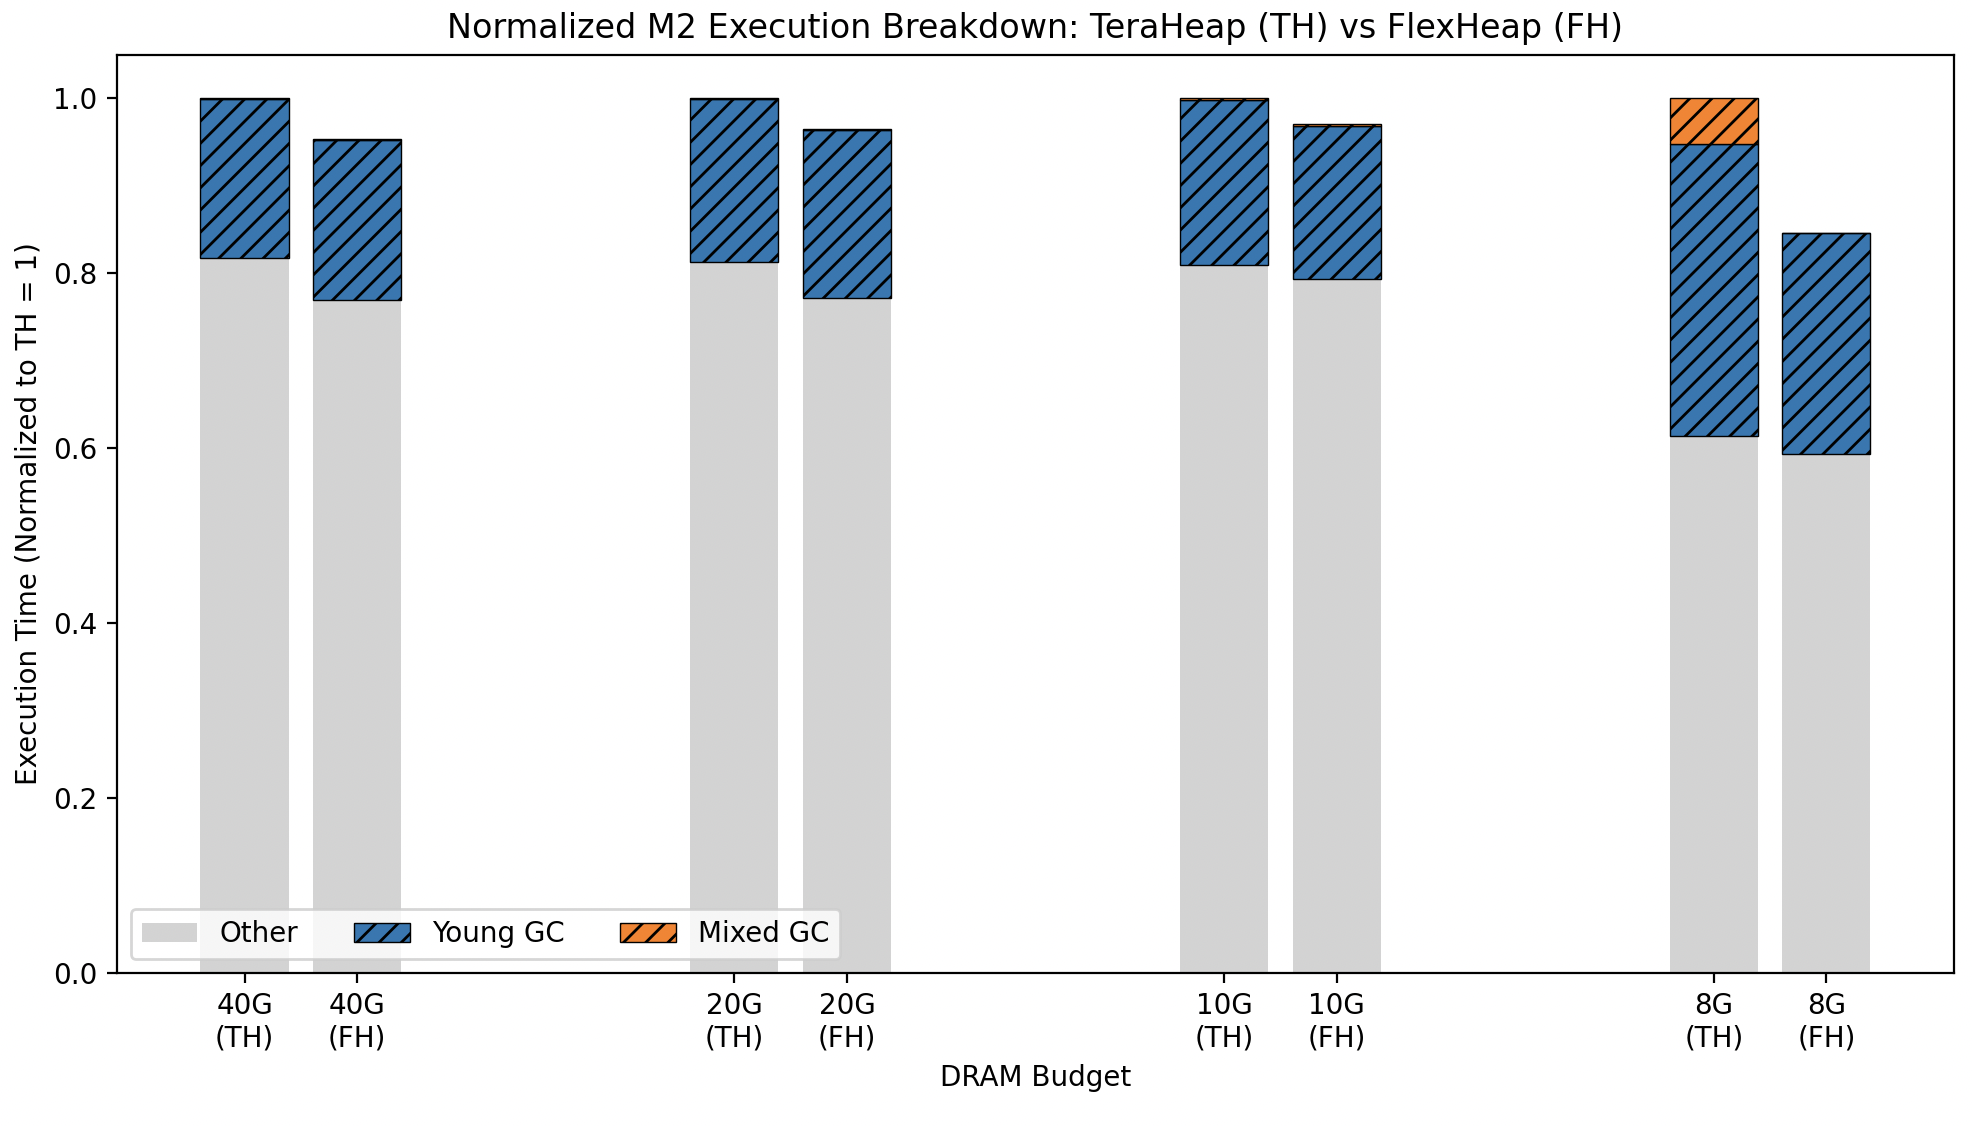
\includegraphics[width=0.95\linewidth]{fig/M2_exec.png}
%   \caption{Normalized execution time breakdown for M2 workload.}
%   \label{fig:m2-exec}
% \end{figure}

% \begin{table}[H]
% \begin{table}[htbp]
% \vspace{1em}
% \centering
% \small
% \renewcommand{\arraystretch}{0.8}
% \caption{Spark benchmark configurations under TeraHeap (static) and FlexHeap (dynamic).}
% \label{tab:spark-benchmark-configs}
% \begin{tabular}{|l|l|c|}
% \hline
% \textbf{Configuration} & \textbf{Benchmark} & \textbf{H1/ H2 Allocation (G)} \\
% \hline
% \multirow{7}{*}{TeraHeap (static)} 
% & PageRank             & 64\,G / 16\,G \\
% & ConnectedComponent   & 68\,G / 16\,G \\
% & ShortestPaths        & 42\,G / 16\,G \\
% & TriangleCount        & 64\,G / 16\,G \\
% & SVDPlusPlus          & 24\,G / 16\,G \\
% & LinearRegression     & 54\,G / 16\,G \\
% & LogisticRegression   & 54\,G / 16\,G \\
% \hline
% \multirow{7}{*}{FlexHeap (dynamic)} 
% & PageRank             & 74\,G / 6\,G  \\
% & ConnectedComponent   & 80\,G / 4\,G  \\
% & ShortestPaths        & 50\,G / 8\,G \\
% & TriangleCount        & 64\,G / 16\,G \\
% & SVDPlusPlus          & 28\,G / 12\,G \\
% & LinearRegression     & 64\,G / 6\,G  \\
% & LogisticRegression   & 60\,G / 10\,G \\
% \hline
% \end{tabular}
% \end{table}
%
%
% \begin{table*}[!t]
% % \begin{table}[!htbp]
% % \begin{center}
% \renewcommand{\arraystretch}{1.3}
% \resizebox{\textwidth}{!}{%
% \begin{tabular}{|l|c|c|c|c|c|c|c|}
% \hline
% \textbf{Configuration} & \textbf{PageRank} & \textbf{ConnectedComponent} & \textbf{ShortestPaths} & \textbf{TriangleCount} & \textbf{SVDPlusPlus} & \textbf{LinearRegression} & \textbf{LogisticRegression} \\
% \hline
% TeraHeap (static DRAM) & 64G H1 / 16G H2 & 68G H1 / 16G H2 & 68G H1 / 16G H2 & 64G H1 / 16G H2 & 24G H1 / 16G H2 & 54G H1 / 16G H2 & 54G H1 / 16G H2 \\
% \hline
% FlexHeap               & 74G H1 / 6G H2  & 80G H1 / 4G H2  & 48G H1 / 10G H2 & 64G H1 / 16G H2 & 28G H1/ 12G H2 & 64G H1/ 6G H2 & 60G H1/ 10G H2  \\
% \hline
% \end{tabular}
% }
% \caption{Spark benchmarks under two configurations: TeraHeap with static DRAM partitioning and FlexHeap.}
% \label{tab:spark-benchmark-configs}
% % \end{center}
% \end{table*}
% \vspace{-1em}  % optional: reduce whitespace
%


